\apendice{Documentación técnica de programación}

\section{Introducción}
En este apartado se detallará cómo entrenar nuestros agentes inteligentes y como hacerlos funcionar en el entorno del videojuego. 

\section{Estructura de directorios}
A continuación se va a explicar la estructura de directorios para no perder el tiempo buscándolo todo.

Los principales directorios del proyecto son:
\begin{itemize}
    \item Proyectos Unity
    \item Redes Neuronales
    \item DecicionTreeClasiffiers
    \item Ejemplos y pruebas
\end{itemize}

En el directorio de «proyectos Unity»  encontraremos los dos principales proyectos de videojuego con los que se ha trabajado. En primer lugar podemos encontrar el proyecto «Juego». Este proyecto contiene el juego principal, el que van a utilizar los usuarios para obtener los datos de las partidas. Por otro lado tenemos el proyecto «Juego\_lite». Esta segunda versión de la implementación es una versión reducida del primero, carece de menús y sonido, ya que únicamente está destinado a ser jugado por la máquina. Finalmente tenemos un último directorio en el que encontramos los proyectos de que probaban funcionalidades muy concretas, como las pruebas de conexión de sockets y el lanzamiento del juego con parámetros desde terminal.

En los directorio «DecsionTreeClasiffiers» y «RedesNeuronales», encontramos una \empg{build} del juego lista para funcionar, cada una referente a su tipo de algorimo. Los scripts de Python deben ir dentro del directorio AI\_Data y los modelos entrenados los he colocado junto al ejecutable pero, como se va a referenciar con una ruta relativa, se pueden colocar donde más nos guste. Junto al ejecutable he creado un acceso directo al mismo, esto es porque el juego ha de lanzarse con parámetros y esto nos facilita la tarea.

Como es de esperar, la realización de este proyecto ha requerido de una gran labor de investigación, síntesis y pruebas. En el directorio pruebas y ejemplos podemos encontrar un «batiburrillo» de ejemplos realizados con ayuda del tutor y apuntes de la asignatura de «Minería de datos». Además, se han guardado en ésta carpeta varios sets de datos antiguos que fueron utilizados en las primeras pruebas.


\section{Manual del programador}
Voy a proceder a explicar cómo se debería proceder para la compilación del juego, entrenamiento de los agentes inteligentes y su posterior uso.


\section{Compilación, instalación y ejecución del proyecto}
Como que este proyecto esta dividido en tantas partes empezaré explicando cómo instalar python, qué bibliotecas necesitamos y cómo se instalan.

\subsection{Instalando Python}

Este royecto ha sido realizado utilizando \emph{Anaconda}\footnote{\url{https://www.continuum.io/downloads}}, una distribución de \emph{Python}. Para obtener \emph{Anaconda} vamos a su página web y descargamos la versión correspondiente a nuestro sistema operativo(32/64 bits). 

\begin{figure}[h!]
    \centering
    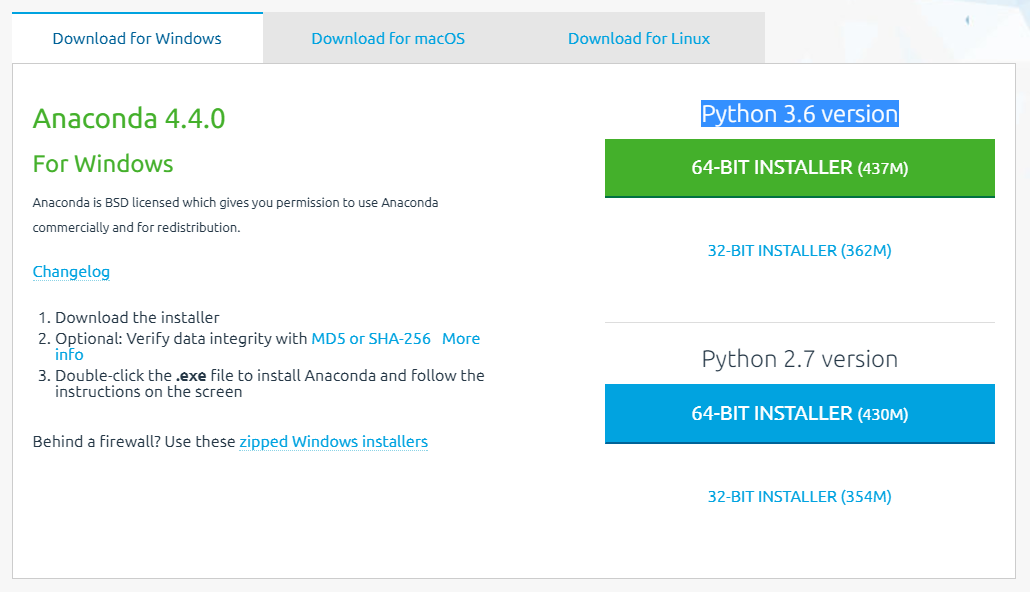
\includegraphics[width=\textwidth]{descargaPython}
    \caption{Descarga Anaconda}
    \label{fig:anaconda}
\end{figure}


IMPORTANTE: Actualmente hay varias versiones disponibles de Python. A lo largo de este proyecto se ha utilizado la 3.5.2, que sería compatible con cualquier versión a partir de la 3.0, pero incompatible con cualquier versión inferior \ref{fig:anaconda}.

Una vez instalado anaconda procedemos a instalar los paquetes necesarios para los scripts. \emph{Anaconda} trae por defecto muchos paquetes de los que necesitamos, ente los que están: 
\begin{itemize}
    \item NumPy.
    \item pandas.
    \item SciPy.
    \item Matplotlib.
    \item Jupyter.
\end{itemize}

Además de estos paquetes, necesitaremos \emph{Pickle} y \emph{Deap}. La instalación de paquetes en \emph{Anaconda} es sumamente sencilla. Abrimos el terminal de windows y escribimos:

\colorbox{black}{\textcolor{white}{conda install package-name}}


Cuando termine de instalar deberíamos tener el entorno de  listo para trabajar en él.

\subsection{Instalando Unity3D}

Para cargar y compilar el juego necesitaremos Unity3D. Es software de desarrollo de videojuegos se puede descargar gratuitamente desde su página web. \url{https://unity3d.com/es/get-unity/download}

\begin{figure}[h!]
    \centering
    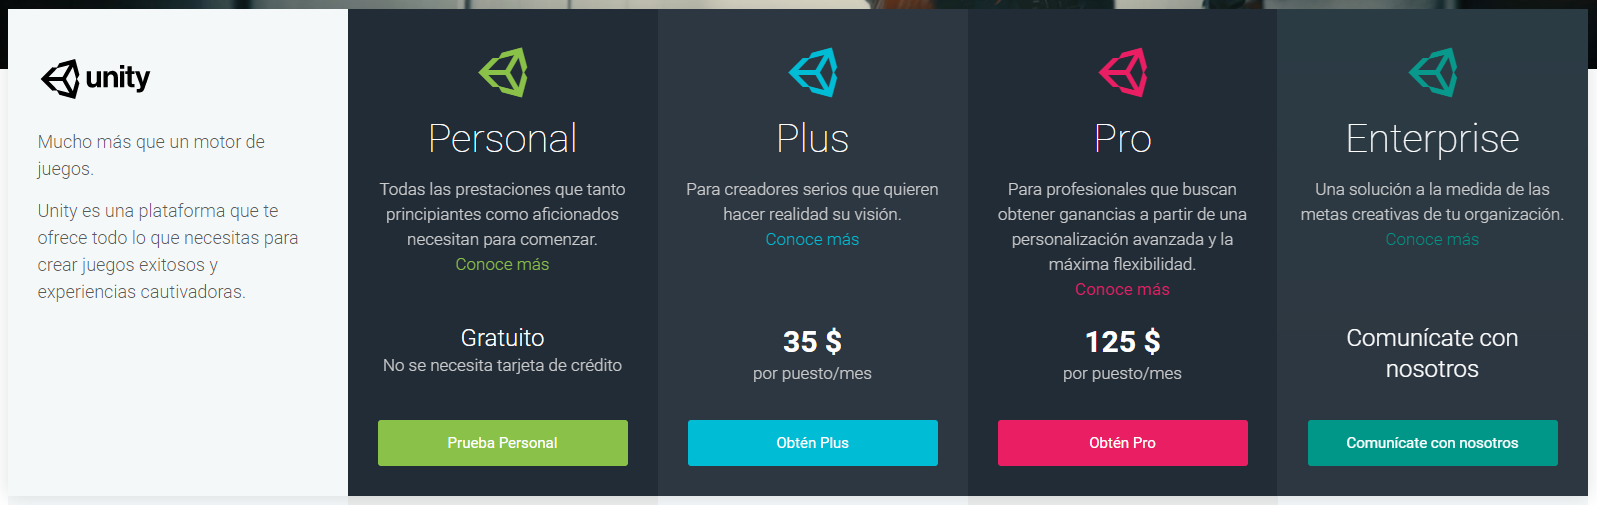
\includegraphics[width=\textwidth]{UnityInstall}
    \caption{Descarga Unity3D}
    \label{fig:Unity}
\end{figure}

Para este proyecto es suficiente con descargar la versión gratuita. Ejecutamos el instalador y elegimos la opción por defecto. En una de las pantallas nos permite seleccionar qué componentes se quiere instalar, con seleccionar los que se ven en \ref{fig:Unity2} es suficiente.

\begin{figure}[h!]
    \centering
    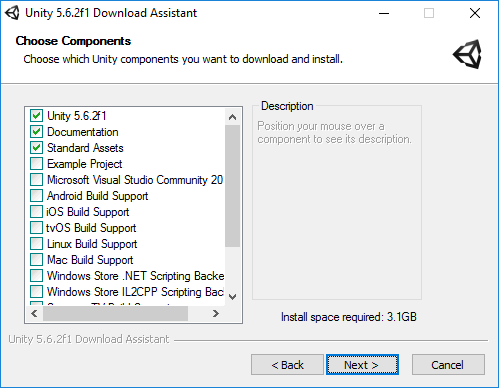
\includegraphics[width=0.5\textwidth]{UnityInstall2}
    \caption{Descarga Unity3D}
    \label{fig:Unity2}
\end{figure}


\subsection{Compilación}
Para la compilación del juego hay que ejecutar Unity3D y cargar el proyecto que se va a compilar. Para ello se han de seguir los siguientes pasos:
\begin{itemize}
    \item 1 - Lanzar Unity3D y cargar el proyecto. Al lanzar Unity3D, si no hemos modificado ninguna configuración, nos debe mostrar una ventana como \ref{fig:compile1}. En esta ventana nos muestra los proyectos recientes que, si es la primera vez que lo lanzamos, estará vacía. Para cargar un proyecto no listado pulsamos el botón «Open» y buscamos el proyecto en nuestro disco. En este caso hay que cargar el que he denominado «Juego».
        \begin{figure}[h!]
        \centering
        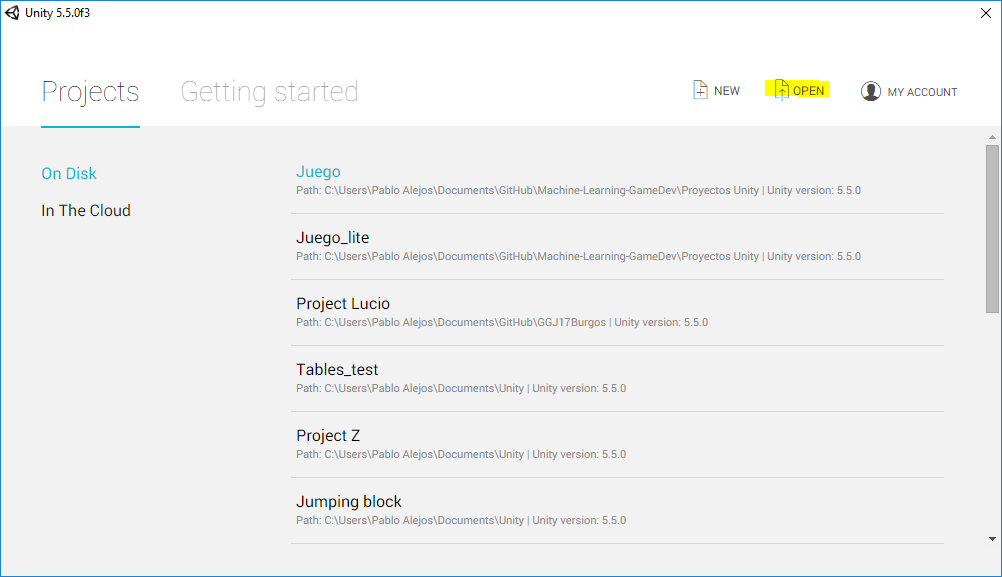
\includegraphics[width=\textwidth]{Compile1}
        \caption{Carga proyecto Unity3D}
        \label{fig:compile1}
        \end{figure}
\item 2- Compilación del juego. Para compilar el juego vamos a «File» > «Build settings» y se nos abre la ventana de compilación \ref{fig:compile3}.
        \begin{figure}[h!]
        \centering
        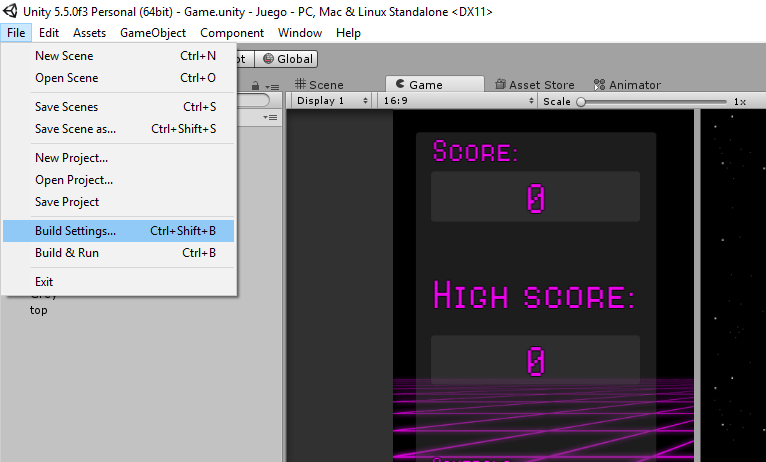
\includegraphics[width=\textwidth]{Compile2}
        \caption{Compilar proyecto}
        \label{fig:compile2}
        \end{figure}
En la ventana de compilación deberían aparecer cargadas dos escenas, identificadas con el id 0 y 1 respectivamente. Hecha esta comprobación procedemos con la \emph{build}. Para compilar el juego pulsamos sobre build y seleccionamos la carpeta donde lo queremos guardar.
        \begin{figure}[h!]
        \centering
        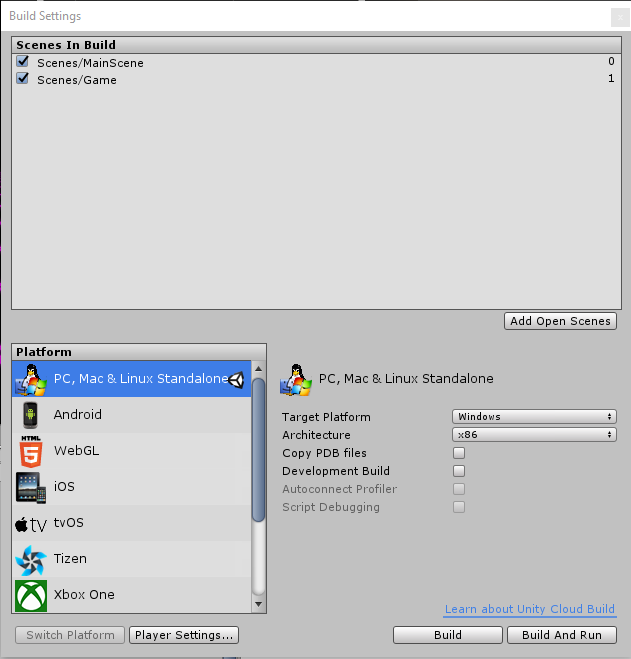
\includegraphics[width=\textwidth]{Compile3}
        \caption{Ventana de compilación}
        \label{fig:compile3}
        \end{figure}
\end{itemize}

Con el juego ya compilado no tendríamos mas que entregar al jugador el ejecutable con las carpeta de binarios generada y este podría empezar a jugar y a generar datos. Mientras nuestro «sujeto de prueba» está entretenido jugando, vamos a continuar haciendo la build del juego que utilizará nuestro agente inteligente.



\subsection{Incorporación de los scripts}
En este punto ya tenemos \emph{Python} instalado, Unity3D instalado y hemos creado una build del juego.

Para la compilación del juego reducido, el juego que utilizarán los agentes inteligentes se siguen los mismos pasos mencionados anteriormente, pero esta vez cargaremos el proyecto denominado «Juego\_lite». Esta es una versión reducida del juego, no dispone de menú principal y de ha eliminado la banda sonora.

Una vez compilado debemos añadir a la build los scripts ............ ... COMPLETAR.



\section{Pruebas del sistema}
